\chapter{Introduction}
\label{chap:introduction}

Third-party libraries are an integral part of many software systems. They could facilitate the implementation of a specific component (code reuse), or even offer an additional functionality, that is only available when using them. Most of these libraries are accessible through their \textit{Application Programming Interface} (API), which may consist of numerous classes and methods. However, it is now clear, based on multiple studies, that APIs lack proper examples and documentation and, in general, sufficient explanation on how to be used \cite{Robillard:2009, Uddin:2015}.

In an attempt to overcome the above mentioned limitations, the developers often exploit general-purpose or specialised search engines (\textit{Code Search Engines} or CSEs), or even \textit{Question-and-Answer} services (Q\&A) such as Stack Overflow\footnote{\url{http://stackoverflow.com/}}, in order to find possible API usages. A noticeable research is conducted in \cite{Hoffmann:2007}, where \nolink{\citeauthor{Hoffmann:2007}} clearly identify the API-related queries as the most common queries on the web, for the Java language. The results of their research are illustrated in \Cref{images:common-queries}\footnote{This figure, as well as small parts of this chapter, have been presented as part of the \textit{Informatics Research Proposal} (IRP) document.}.

\begin{figure}[ht]
  \centering
  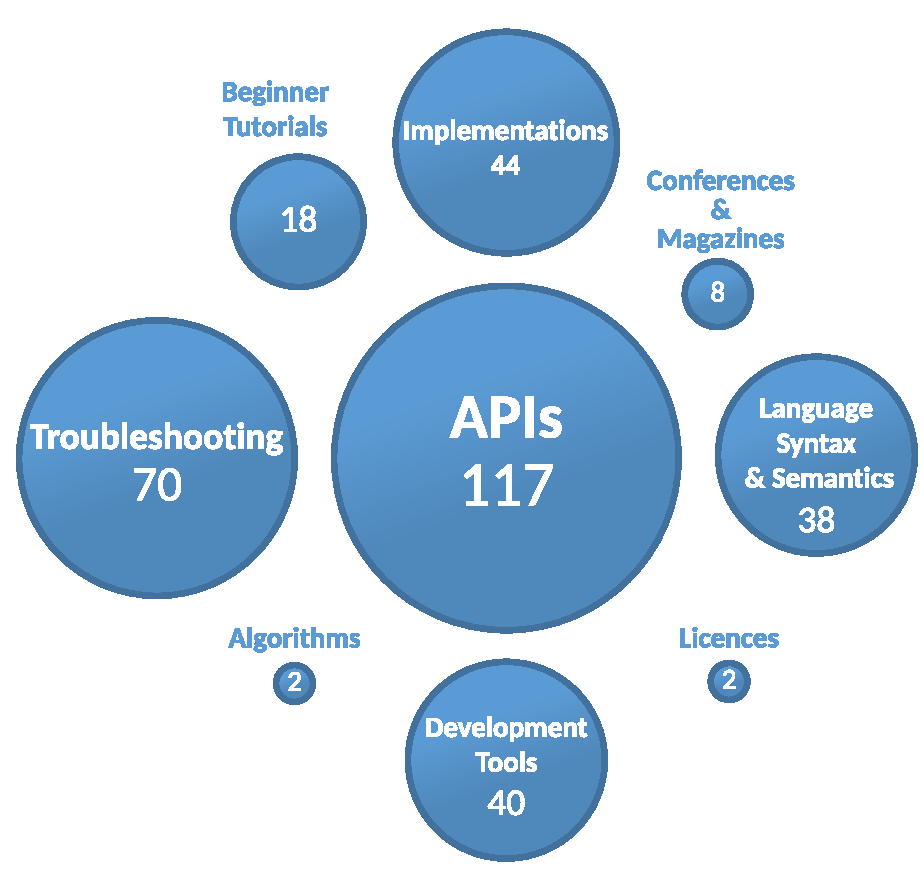
\includegraphics[scale=0.4]{images/common-queries}
  \caption[Most common types of queries initiated by developers on the web]{Most common types of queries initiated by developers on the web.}
  \label{images:common-queries}
\end{figure}


\section{Hypothesis of the Dissertation}
\label{sec:hypothesis}

The purpose of the current dissertation is to summarise typical use cases of an API, by leveraging powerful statistical techniques from the emerging fields of \textit{Machine Learning} (ML) and \textit{Natural Language Processing} (NLP). A potentially successful system would collect API usage examples from the web, apply unsupervised learning techniques to cluster similar examples, and show a representative example from each cluster, summarising in this way the target API.

Interpreting the purpose of this dissertation, our intuition tells us that an API can be effectively summarised using statistical techniques, that may be successfully applied to source code. Although such techniques have been well applied to natural language, their application to source code is quite challenging, as we have to take into account both its semantic context and its structure. Moreover, a key hypothesis of the dissertation is that the presentation of snippets would be of greater value to the developers, than that of API method call sequences.


\section{Motivation of the Dissertation}
\label{sec:motivation}

The benefits of such a system are numerous for the users as well as for the developers of an API. In \cite{Spinellis:2006}, \nolink{\citeauthor{Spinellis:2006}} identifies \textit{time}\footnote{\nolink{\citeauthor{Spinellis:2006}} implies several aspects of time, however, we are mainly interested in the development time in this dissertation.} and \textit{quality} as two of the three main factors that may lead a software project to success\footnote{With \textit{cost} being the third factor.}. A system that efficiently summarises an API could improve both of them. More specifically, the presentation of usage examples to the users would lead to time saving, allowing the developers to spend more time in more useful tasks, while it could also help in improving the software's quality by considering popular usage examples of the API. Additionally, the developers of the library might receive useful statistics about the common usages of their library's API, and proceed to enhancements (e.g. enrich it with more examples, in case they notice that the existing ones are not adequate, or even provide a better documentation). 

Furthermore, we see a possible interesting connection of such a system with a new feature that was added to the popular Q\&A website Stack Overflow. The \textit{Documentation}\footnote{\url{https://stackoverflow.com/documentation}} tool, which is still in Beta mode, is described as a ``community-curated, example-focused developer documentation'', and aims to collect examples that could be used for documentation purposes in different technologies. We argue that a system that performs API usage mining could act as a driving force for the tool, by bootstrapping the examples. Then, the users of the Documentation could improve them, while adding the appropriate descriptive text.

Finally, there is an additional motivation, which stems from a novel evaluation approach presented in \cite{{Fowkes2:2015}}. There, \nolink{\citeauthor{Fowkes2:2015}} evaluate the quality of the patterns -in the form of API call sequences- mined by systems that perform API usage mining, using the \texttt{examples} directory that possibly exists in the repository of the target library. This approach has not been applied to source code yet, though, and we are interested in doing so in this project.


\section{Possible Usage Scenarios}
\label{sec:use-case-scenarions}

We may think of several usage scenarios for the system to be developed. Below we analyse two typical use cases, as well as a brainstorming one.

\begin{itemize}
\item The most typical usage scenario involves the expansion of an API's documentation. For instance, the \textit{APIMiner}\footnote{\url{http://apiminer.org/}} tool augments the documentation of the Android API with source code examples.
\item Another common scenario is that of a CSE, that is specialised to APIs. As an example, we mention the \textit{Codota}\footnote{\url{http://www.codota.com/}} and the KodeBeagle\footnote{\url{http://kodebeagle.com/}} CSEs. Such a CSE could also propose similar examples, or even API methods that are often invoked together.
\item A more brainstorming scenario has been described in \Cref{sec:motivation}, and makes use of the new StackOverflow's \textit{Documentation} feature. That is, the system could be exploited with the purpose of augmenting the Documentation with examples.
\end{itemize}


\section{Structure of the Dissertation}
\label{sec:structure}

The rest of this report is organised as follows: In \Cref{chap:background} we set the appropriate background, by introducing terms and techniques that are going to be mentioned during the analysis of our implementation. Then, in \Cref{chap:existing-work}, we define the problem faced in this dissertation, while providing an overview of the state-of-the-art systems that perform API usage mining, with the aim to present usage examples to the users. \Cref{chap:conceptual-design-work} describes the approach and the methodology followed in order to solve the problem, as well as in order to tackle any obstacles, before analysing the actual implementation of the system in \Cref{chap:implementation}. There, we extensively analyse each component of the system, and any algorithms implemented and used from our system. That chapter is followed by \Cref{chap:evaluation}, where we describe the evaluation methodology, in terms of the metrics used and the experiments conducted, while presenting and interpreting the results. Finally, in \Cref{chap:conclusion} we present the contributions and limitations of this work, and suggest possible enhancements. For the sake of a better understanding of the implementation, as well as of the experiments' results, additional material, including indicative snippets that are mined by our system, are presented in the appendices. 